\documentclass[tikz,convert=false]{standalone}
\usetikzlibrary{er}
\begin{document}
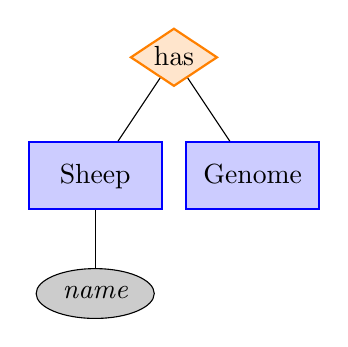
\begin{tikzpicture}[text depth=1pt,%
  every attribute/.style={fill=black!20,draw=black},%
  every entity/.style={fill=blue!20,draw=blue,thick},%
  every relationship/.style={fill=orange!20,draw=orange,%
  thick,aspect=1.5}]

  \node [entity] (sheep) at (0,0) {Sheep}
    child {node [key attribute] {name}};
  \node [entity] (genome) at (2,0) {Genome};
  \node [relationship] at (1,1.5) {has}
    edge (sheep)
    edge (genome);
\end{tikzpicture}
\end{document}
